\documentclass[crop,tikz]{standalone}
\usepackage{physics}
\usetikzlibrary{positioning}

\begin{document}
        \tikzset{font={\fontsize{8pt}{12}\selectfont}}
        \begin{tikzpicture}
                \node at (0, 0) {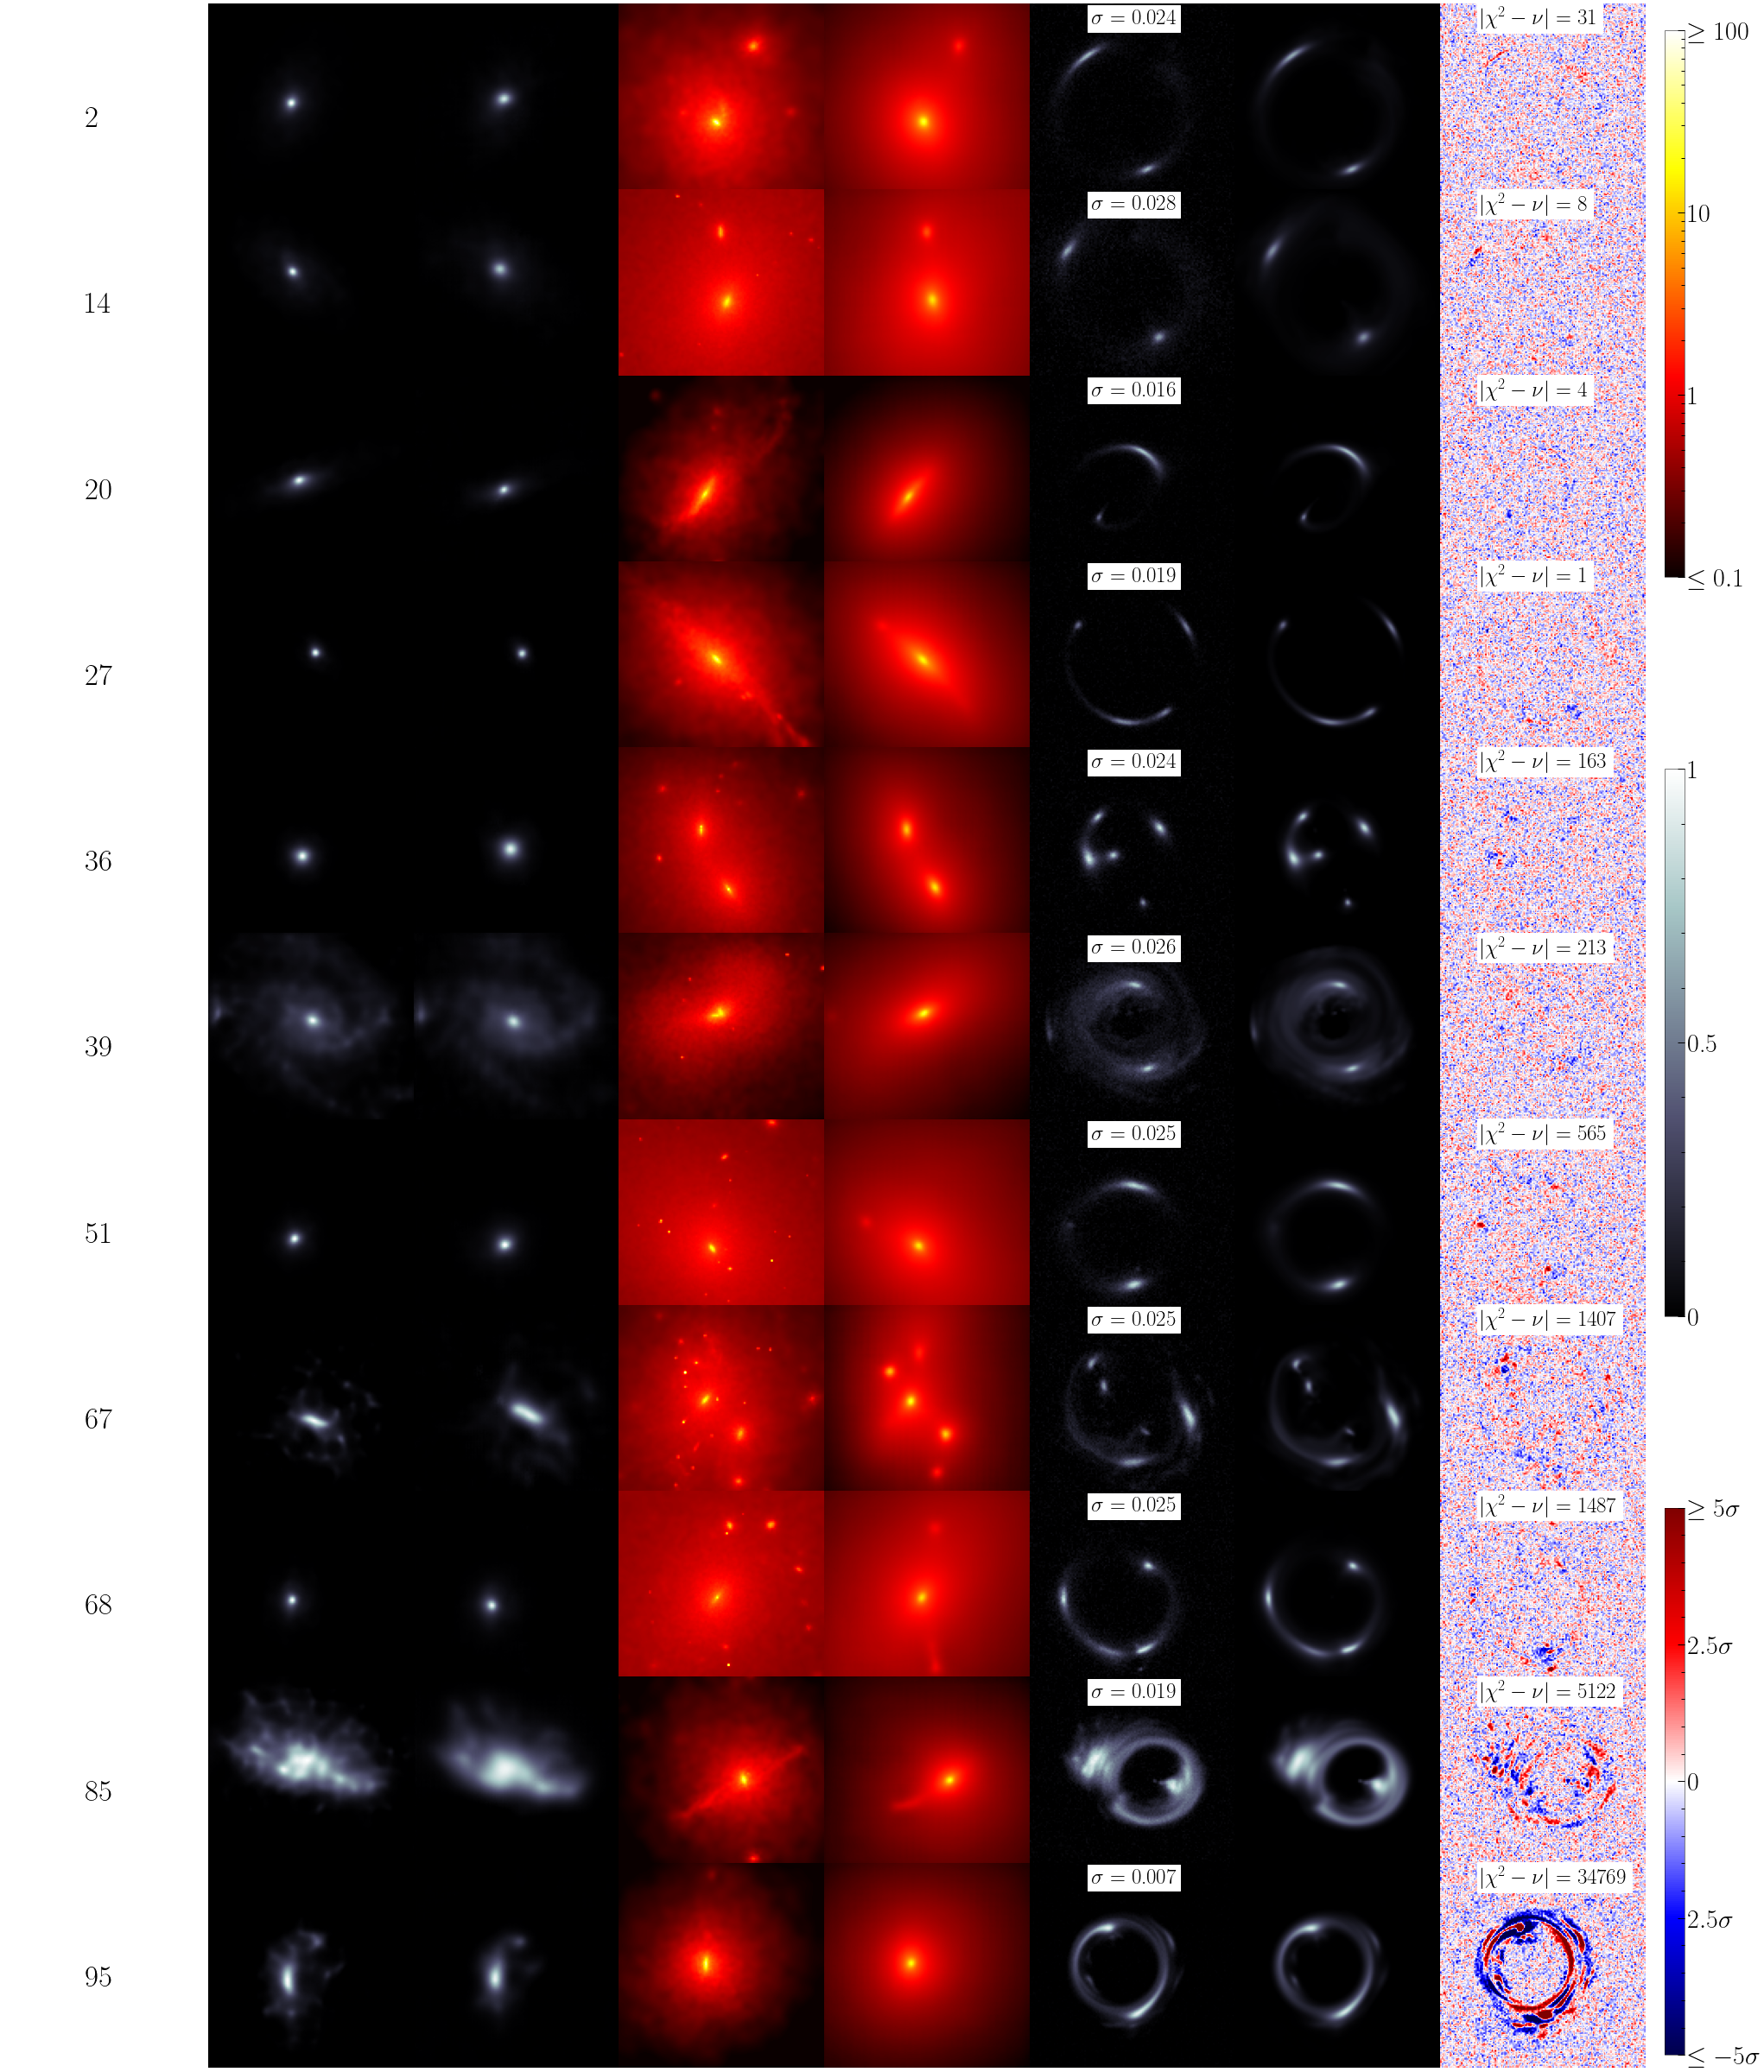
\includegraphics[width=18cm]{ewc_representative_sample}};
                % without Power spectrum
                \node at (-8, 10.8) {Percentile};
                \node at (-4.8, 11.3) {Source};
                \node at (-5.8, 10.8) {COSMOS};
                \node at (-3.8, 10.8) {RIM+FT};
                \node at (-0.6, 11.3) {Convergence};
                \node at (-1.6, 10.8) {IllustrisTNG};
                \node at (0.4, 10.8) {RIM+FT};
                \node at (2.6,   10.8) {Observation};
                \node at (4.6, 10.8) {RIM+FT};
                \node at (6.8, 10.8) {Residuals};
                \draw[dashed] (-9, -8.5) -- (-7, -8.5); 
                \node at (-8, -8.7) {SNR $> 22\,\mathrm{dB}$};
                \node[rotate=-90] at (9.2, 0) {Intensity};
                \node[rotate=-90] at (9.2, 7.8) {Convergence};
                \node[rotate=-90] at (9.2, -7.8) {Residuals};

                % With power spectrum
                %\node at (-8, 10.5) {Percentile};
                %\node at (-5.2, 11.2) {Source};
                %\node at (-6.2, 10.5) {COSMOS};
                %\node at (-4.4, 10.5) {RIM+FT};
                %\node at (-1.4, 11.2) {Convergence};
                %\node at (-2.4, 10.5) {IllustrisTNG};
                %\node at (-0.6, 10.5) {RIM+FT};
                %\node at (1., 10.5) {Observation};
                %\node at (3.6, 10.5) {RIM+FT};
                %\node at (5.8, 10.5) {Residuals};
                %\draw[dashed] (-9, -8.5) -- (-7, -8.5); 
                %\node at (-8, -8.7) {SNR $> 22\,\mathrm{dB}$};
                %\node[rotate=-90] at (9.2, 0) {Intensity};
                %\node[rotate=-90] at (9.2, 8) {Convergence};
                %\node[rotate=-90] at (9.2, -8) {Residuals};
        \end{tikzpicture}
\end{document}
